% questions.tex —— 2013 年全国Ⅱ卷（理科） · 题目内容片段（无答案）
% 由 tools/generate_projects.py 依来源总账自 2013/2013_数学真题_全国2理_试题.md 生成，勿手改（改源 MD 后重跑）


\gkpart{数学}

\begin{gktip}
\textbf{来源说明}：本题面依据固定源 PDF 两页 A3 题面逐题转录，原卷印刷页码 829–830。固定源只含试题和作答空白，不附答案或解析；答案和解析均由本库独立复算。

\textbf{图形说明}：第 6、7、18、19、22 题的题面图形在 LaTeX 工程中以 TikZ 矢量源重绘。题面中的图片标记仅为转换器定位这些矢量源的标记，仓库不保存 PNG、JPEG 或 SVG 图形文件。

\textbf{栏目说明}：固定源按选择题 1–12、填空题 13–16、解答题 17–24 连续排印；第 22–24 题的选考或作答属性为“题面未给规则”，本转录不补写任选或必答规则。
\end{gktip}

\gkpart{一、选择题}

\begin{question}
\gkti{1}已知集合 $M=\{x\mid(x-1)^2<4,\ x\in\mathbb R\}$，$N=\{-1,0,1,2,3\}$，则 $M\cap N=$\mbox{（　　）}

（A）$\{0,1,2\}$　　（B）$\{-1,0,1,2\}$　　（C）$\{-1,0,2,3\}$　　（D）$\{0,1,2,3\}$

\end{question}
\begin{question}
\gkti{2}设复数 $z$ 满足 $(1-i)z=2i$，则 $z=$\mbox{（　　）}

（A）$-1+i$　　（B）$-1-i$　　（C）$1+i$　　（D）$1-i$

\end{question}
\begin{question}
\gkti{3}等比数列 $\{a_n\}$ 的前 $n$ 项和为 $S_n$，已知 $S_3=a_2+10a_1$，$a_5=9$，则 $a_1=$\mbox{（　　）}

（A）$\dfrac13$　　（B）$-\dfrac13$　　（C）$\dfrac19$　　（D）$-\dfrac19$

\end{question}
\begin{question}
\gkti{4}已知 $m,n$ 为异面直线，$m\perp$ 平面 $\alpha$，$n\perp$ 平面 $\beta$。直线 $l$ 满足 $l\perp m$，$l\perp n$，$l\not\subset\alpha$，$l\not\subset\beta$，则\mbox{（　　）}

（A）$\alpha\parallel\beta$ 且 $l\parallel\alpha$　　（B）$\alpha\perp\beta$ 且 $l\perp\beta$

（C）$\alpha$ 与 $\beta$ 相交，且交线垂直于 $l$　　（D）$\alpha$ 与 $\beta$ 相交，且交线平行于 $l$

\end{question}
\begin{question}
\gkti{5}已知 $(1+ax)(1+x)^5$ 的展开式中 $x^2$ 的系数为 $5$，则 $a=$\mbox{（　　）}

（A）$-4$　　（B）$-3$　　（C）$-2$　　（D）$-1$

\Needspace{0.4\textheight}
\end{question}
\begin{question}
\gkti{6}执行如图的程序框图，如果输入的 $N=10$，那么输出的 $S=$\mbox{（　　）}
\nopagebreak[4]
\begin{center}% 2013 全国卷Ⅱ理科第 6 题：阶乘倒数累加程序框图。
\begin{tikzpicture}[font=\footnotesize, >=Stealth, node distance=4mm, line width=0.4pt,
  box/.style={draw, minimum height=1.65em, minimum width=8.0em, inner xsep=4pt},
  term/.style={draw, rounded corners=6pt, minimum height=1.65em, inner xsep=8pt},
  io/.style={draw, trapezium, trapezium left angle=70, trapezium right angle=110,
             minimum height=1.65em, inner xsep=4pt},
  dec/.style={draw, diamond, aspect=2.25, inner sep=1.6pt}]
  \node[term] (start) {开始};
  \node[io, below=of start] (input) {输入 $N$};
  \node[box, below=of input] (init) {$k=1,\ S=0,\ T=1$};
  \node[box, below=of init] (divide) {$T=\dfrac{T}{k}$};
  \node[box, below=of divide] (sum) {$S=S+T$};
  \node[box, below=of sum] (inc) {$k=k+1$};
  \node[dec, below=7mm of inc] (cond) {$k>N$};
  \node[io, below=8mm of cond] (output) {输出 $S$};
  \node[term, below=of output] (end) {结束};
  \draw[->] (start)--(input)--(init)--(divide)--(sum)--(inc)--(cond);
  \draw[->] (cond.south)--node[right] {是}(output);
  \draw[->] (output)--(end);
  \draw[->] (cond.east)-| node[pos=0.18,above] {否} ($(divide.east)+(12mm,0)$) |- (divide.east);
\end{tikzpicture}
\end{center}
\nopagebreak[4]
（A）$1+\dfrac12+\dfrac13+\cdots+\dfrac1{10}$　　（B）$1+\dfrac1{2!}+\dfrac1{3!}+\cdots+\dfrac1{10!}$

（C）$1+\dfrac12+\dfrac13+\cdots+\dfrac1{11}$　　（D）$1+\dfrac1{2!}+\dfrac1{3!}+\cdots+\dfrac1{11!}$

\Needspace{0.4\textheight}
\end{question}
\begin{question}
\gkti{7}一个四面体的顶点在空间直角坐标系 $O-xyz$ 中的坐标分别是 $(1,0,1)$，$(1,1,0)$，$(0,1,1)$，$(0,0,0)$。画该四面体三视图中的正视图时，以 $zOx$ 平面为投影面，则得到正视图可以为\mbox{（　　）}
\nopagebreak[4]
\begin{center}% 2013 全国卷Ⅱ理科第 7 题：四面体正视图四个选项；虚线表示隐藏棱。
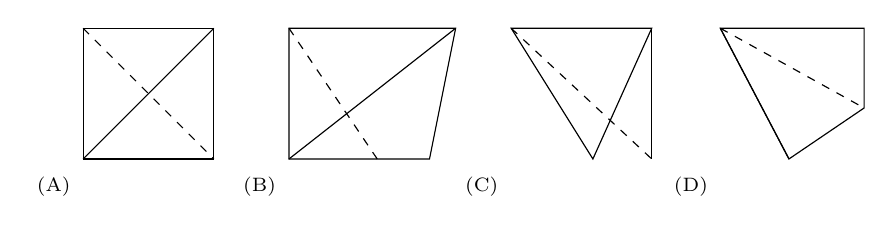
\begin{tikzpicture}[font=\scriptsize, line width=0.42pt, scale=0.83]
  % A
  \begin{scope}
    \node at (-0.45,-0.42) {(A)};
    \draw (0,0)--(2,0)--(2,2)--(0,2)--cycle;
    \draw (0,0)--(2,2);
    \draw[dashed] (0,2)--(2,0);
  \end{scope}
  % B
  \begin{scope}[xshift=3.15cm]
    \node at (-0.45,-0.42) {(B)};
    \draw (0,0)--(2.15,0)--(2.55,2)--(0,2)--cycle;
    \draw (0,0)--(2.55,2);
    \draw[dashed] (0,2)--(1.35,0);
  \end{scope}
  % C
  \begin{scope}[xshift=6.55cm]
    \node at (-0.45,-0.42) {(C)};
    \draw (0,2)--(2.15,2)--(1.25,0)--cycle;
    \draw (2.15,2)--(2.15,0);
    \draw[dashed] (0,2)--(2.15,0);
  \end{scope}
  % D
  \begin{scope}[xshift=9.75cm]
    \node at (-0.45,-0.42) {(D)};
    \draw (0,2)--(2.20,2)--(2.20,0.78)--(1.05,0)--cycle;
    \draw (0,2)--(1.05,0);
    \draw[dashed] (0,2)--(2.20,0.78);
  \end{scope}
\end{tikzpicture}
\end{center}
\nopagebreak[4]
\end{question}
\begin{question}
\gkti{8}设 $a=\log_3 6$，$b=\log_5 10$，$c=\log_7 14$，则\mbox{（　　）}

（A）$c>b>a$　　（B）$b>c>a$　　（C）$a>c>b$　　（D）$a>b>c$

\end{question}
\begin{question}
\gkti{9}已知 $a>0$，$x,y$ 满足约束条件

\nopagebreak[4]
\[
\begin{cases}
x\geqslant1,\\
x+y\leqslant3,\\
y\geqslant a(x-3),
\end{cases}
\]

若 $z=2x+y$ 的最小值为 $1$，则 $a=$\mbox{（　　）}

（A）$\dfrac14$　　（B）$\dfrac12$　　（C）$1$　　（D）$2$

\end{question}
\begin{question}
\gkti{10}已知函数 $f(x)=x^3+ax^2+bx+c$，下列结论中错误的是\mbox{（　　）}

（A）$\exists x_0\in\mathbb R,\ f(x_0)=0$

（B）函数 $y=f(x)$ 的图象是中心对称图形

（C）若 $x_0$ 是 $f(x)$ 的极小值点，则 $f(x)$ 在区间 $(-\infty,x_0)$ 单调递减

（D）若 $x_0$ 是 $f(x)$ 的极值点，则 $f'(x_0)=0$

\end{question}
\begin{question}
\gkti{11}设抛物线 $C:y^2=2px\ (p>0)$ 的焦点为 $F$，点 $M$ 在 $C$ 上，$|MF|=5$。若以 $MF$ 为直径的圆过点 $(0,2)$，则 $C$ 的方程为\mbox{（　　）}

（A）$y^2=4x$ 或 $y^2=8x$　　（B）$y^2=2x$ 或 $y^2=8x$

（C）$y^2=4x$ 或 $y^2=16x$　　（D）$y^2=2x$ 或 $y^2=16x$

\end{question}
\begin{question}
\gkti{12}已知点 $A(-1,0)$，$B(1,0)$，$C(0,1)$，直线 $y=ax+b\ (a>0)$ 将 $\triangle ABC$ 分割为面积相等的两部分，则 $b$ 的取值范围是\mbox{（　　）}

（A）$(0,1)$　　（B）$\left(1-\dfrac{\sqrt2}{2},\dfrac12\right)$

（C）$\left(1-\dfrac{\sqrt2}{2},\dfrac13\right]$　　（D）$\left[\dfrac13,\dfrac12\right)$

\end{question}
\gkpart{二、填空题}

\begin{question}
\gkti{13}已知正方形 $ABCD$ 的边长为 $2$，$E$ 为 $CD$ 的中点，则 $\overrightarrow{AE}\cdot\overrightarrow{BD}=$\gkblank{}。

\end{question}
\begin{question}
\gkti{14}从 $n$ 个正整数 $1,2,\cdots,n$ 中任意取出两个不同的数，若取出的两数之和等于 $5$ 的概率为 $\dfrac1{14}$，则 $n=$\gkblank{}。

\end{question}
\begin{question}
\gkti{15}设 $\theta$ 为第二象限角，若 $\tan\left(\theta+\dfrac\pi4\right)=\dfrac12$，则 $\sin\theta+\cos\theta=$\gkblank{}。

\end{question}
\begin{question}
\gkti{16}等差数列 $\{a_n\}$ 的前 $n$ 项和为 $S_n$，已知 $S_{10}=0$，$S_{15}=25$，则 $nS_n$ 的最小值为\gkblank{}。

\end{question}
\gkpart{三、解答题}

\begin{question}
\gkti{17}$\triangle ABC$ 的内角 $A,B,C$ 的对边分别为 $a,b,c$，已知 $a=b\cos C+c\sin B$。

(1) 求 $B$；

(2) 若 $b=2$，求 $\triangle ABC$ 面积的最大值。

\Needspace{0.4\textheight}
\end{question}
\begin{question}
\gkti{18}如图，直三棱柱 $ABC-A_1B_1C_1$ 中，$D,E$ 分别是 $AB,BB_1$ 的中点，$AA_1=AC=CB=\dfrac{\sqrt2}{2}AB$。
\nopagebreak[4]
\begin{center}% 2013 全国卷Ⅱ理科第 18 题：直三棱柱 ABC-A_1B_1C_1，D、E 为中点。
\begin{tikzpicture}[font=\footnotesize, line width=0.45pt]
  \coordinate (A) at (0,0);
  \coordinate (B) at (1.25,-1.25);
  \coordinate (C) at (4.25,0);
  \coordinate (A1) at (0,3.70);
  \coordinate (B1) at (2.15,2.00);
  \coordinate (C1) at (4.25,3.70);
  \coordinate (D) at ($(A)!0.5!(B)$);
  \coordinate (E) at ($(B)!0.5!(B1)$);
  % 可见棱和题中出现的截线。
  \draw (A)--(A1)--(C1)--(C)--cycle;
  \draw (A1)--(B1)--(C1) (B)--(B1);
  \draw (A1)--(D)--(C) (A1)--(E)--(C);
  % 透明棱与被遮挡的辅助关系。
  \draw[dashed] (A)--(B)--(C) (A)--(C) (A1)--(C) (D)--(E);
  \node[below left] at (A) {$A$};
  \node[below] at (B) {$B$};
  \node[below right] at (C) {$C$};
  \node[above left] at (A1) {$A_1$};
  \node[above] at (B1) {$B_1$};
  \node[above right] at (C1) {$C_1$};
  \node[below left] at (D) {$D$};
  \node[left] at (E) {$E$};
\end{tikzpicture}
\end{center}
\nopagebreak[4]
(1) 证明：$BC_1\parallel$ 平面 $A_1CD$；

(2) 求二面角 $D-A_1C-E$ 的正弦值。

\Needspace{0.4\textheight}
\end{question}
\begin{question}
\gkti{19}经销商经销某种农产品，在一个销售季度内，每售出 $1\ \mathrm t$ 该产品获利润 $500$ 元，未售出的产品，每 $1\ \mathrm t$ 亏损 $300$ 元。根据历史资料，得到销售季度内市场需求量的频率分布直方图，如图所示。经销商为下一个销售季度购进了 $130\ \mathrm t$ 该农产品。以 $X$（单位：$\mathrm t$，$100\leqslant X\leqslant150$）表示下一个销售季度内的市场需求量，$T$（单位：元）表示下一个销售季度内经销该农产品的利润。
\nopagebreak[4]
\begin{center}% 2013 全国卷Ⅱ理科第 19 题：频率分布直方图。
\begin{tikzpicture}[font=\footnotesize, >=Stealth, line width=0.42pt, scale=0.75, transform shape, x=0.18cm, y=105cm]
  \draw[->] (-12,0)--(58,0) node[right,align=center] {市场需求量};
  \draw[->] (-10,0)--(-10,0.038) node[above,align=center] {频率\\组距};
  % 坐标轴在 0 与 100 之间的截断符号。
  \draw (-7.8,0.0007)--(-7.0,-0.0007)--(-6.2,0.0007)--(-5.4,-0.0007)--(-4.6,0.0007);
  \draw[dashed] (-10,0.010)--(0,0.010); \node[left,xshift=-1mm] at (-10,0.010) {0.010};
  \draw[dashed] (-10,0.015)--(40,0.015); \node[left,xshift=-1mm] at (-10,0.015) {0.015};
  \draw[dashed] (-10,0.020)--(10,0.020); \node[left,xshift=-1mm] at (-10,0.020) {0.020};
  \draw[dashed] (-10,0.025)--(30,0.025); \node[left,xshift=-1mm] at (-10,0.025) {0.025};
  \draw[dashed] (-10,0.030)--(20,0.030); \node[left,xshift=-1mm] at (-10,0.030) {0.030};
  \draw (0,0) rectangle (10,0.010);
  \draw (10,0) rectangle (20,0.020);
  \draw (20,0) rectangle (30,0.030);
  \draw (30,0) rectangle (40,0.025);
  \draw (40,0) rectangle (50,0.015);
  \node[below] at (-10,0) {$0$};
  \foreach \x/\lab in {0/100,10/110,20/120,30/130,40/140,50/150}
    \node[below] at (\x,0) {\lab};
\end{tikzpicture}
\end{center}
\nopagebreak[4]
(1) 将 $T$ 表示为 $X$ 的函数；

(2) 根据直方图估计利润 $T$ 不少于 $57000$ 元的概率；

(3) 在直方图的需求量分组中，以各组的区间中点值代表该组的各个值，需求量落入该区间的频率作为需求量取该区间中点值的概率（例如：若需求量 $X\in[100,110)$，则取 $X=105$，且 $X=105$ 的概率等于需求量落入 $[100,110)$ 的频率），求 $T$ 的数学期望。

\end{question}
\begin{question}
\gkti{20}平面直角坐标系 $xOy$ 中，过椭圆 $M:\dfrac{x^2}{a^2}+\dfrac{y^2}{b^2}=1\ (a>b>0)$ 右焦点的直线 $x+y-\sqrt3=0$ 交 $M$ 于 $A,B$ 两点，$P$ 为 $AB$ 的中点，且 $OP$ 的斜率为 $\dfrac12$。

(1) 求 $M$ 的方程；

(2) $C,D$ 为 $M$ 上两点，若四边形 $ACBD$ 的对角线 $CD\perp AB$，求四边形 $ACBD$ 面积的最大值。

\end{question}
\begin{question}
\gkti{21}已知函数 $f(x)=e^x-\ln(x+m)$。

(1) 设 $x=0$ 是 $f(x)$ 的极值点，求 $m$，并讨论 $f(x)$ 的单调性；

(2) 当 $m\leqslant2$ 时，证明 $f(x)>0$。

\Needspace{0.4\textheight}
\end{question}
\begin{question}
\gkti{22}如图，$CD$ 为 $\triangle ABC$ 外接圆的切线，$AB$ 的延长线交直线 $CD$ 于点 $D$，$E,F$ 分别为弦 $AB$ 与弦 $AC$ 上的点，且 $BC\cdot AE=DC\cdot AF$，$B,E,F,C$ 四点共圆。
\nopagebreak[4]
\begin{center}% 2013 全国卷Ⅱ理科第 22 题：外接圆、切线及过 B,E,F,C 的圆。
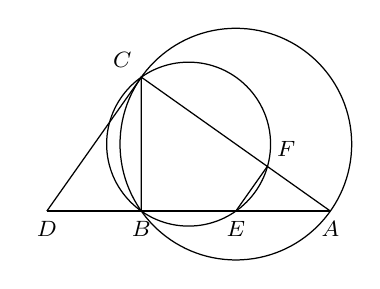
\begin{tikzpicture}[font=\footnotesize, line width=0.45pt]
  \coordinate (B) at (0,0);
  \coordinate (E) at (1.20,0);
  \coordinate (A) at (2.40,0);
  \coordinate (D) at (-1.20,0);
  \coordinate (C) at (0,1.70);
  \coordinate (F) at (1.60,0.567);
  \coordinate (O) at (1.20,0.85);
  \coordinate (o) at (0.60,0.85);
  \draw (O) circle[radius=1.471];
  \draw (o) circle[radius=1.041];
  \draw (D)--(A);
  \draw (D)--(C);
  \draw (B)--(C)--(A);
  \draw (E)--(F);
  \node[below] at (D) {$D$};
  \node[below] at (B) {$B$};
  \node[below] at (E) {$E$};
  \node[below] at (A) {$A$};
  \node[above left] at (C) {$C$};
  \node[above right] at (F) {$F$};
\end{tikzpicture}
\end{center}
\nopagebreak[4]
(1) 证明：$CA$ 是 $\triangle ABC$ 外接圆的直径；

(2) 若 $DB=BE=EA$，求过 $B,E,F,C$ 四点的圆的面积与 $\triangle ABC$ 外接圆面积的比值。

\end{question}
\begin{question}
\gkti{23}已知动点 $P,Q$ 都在曲线 $C:\begin{cases}x=2\cos t,\\y=2\sin t,\end{cases}\ (t$ 为参数$)$ 上，对应参数分别为 $t=\alpha$ 与 $t=2\alpha\ (0<\alpha<2\pi)$，$M$ 为 $PQ$ 的中点。

(1) 求 $M$ 的轨迹的参数方程；

(2) 将 $M$ 到坐标原点的距离 $d$ 表示为 $\alpha$ 的函数，并判断 $M$ 的轨迹是否经过坐标原点。

\end{question}
\begin{question}
\gkti{24}设 $a,b,c$ 均为正数，且 $a+b+c=1$，证明：

(1) $ab+bc+ca\leqslant\dfrac13$；

(2) $\dfrac{a^2}{b}+\dfrac{b^2}{c}+\dfrac{c^2}{a}\geqslant1$。

\end{question}